\section{Introduction}
The success of any complex software-intensive system is dependent on how effectively it addresses the stakeholder's quality attribute concerns such as security, usability, availability, and interoperability. Designing a system to satisfy these concerns involves devising and comparing alternate solutions, understanding their trade-offs, and ultimately making a series of design choices. These architectural decisions typically begin with design primitives such as architectural tactics and patterns.

Tactics are the building blocks of architectural design~\cite{bass:arch12}, reflecting the fundamental choices that an architect makes to address a quality attribute concern. Architectural tactics come in many different shapes and sizes and describe solutions for a wide range of quality concerns. Architectural tactics are particularly prevalent across high-performance and fault tolerant software systems. Reliability tactics such as Redundancy with Voting, Heartbeat, and Check-Pointing provide solutions for fault mitigation, detection, and recovery. Performance tactics such as Resource Pooling and Scheduling help optimize response time and latency.


%% When the paper gets accepted, change the wording to no long refer to ourselves in the 3rd person

%%% Build up the previous study and show how important/profound it was. This will make our work seem more important

%%%The importance of rigorously and robustly implementing architectural tactics was highlighted by a small study conducted in an important previous work which investigated tactic implementations in Hadoop and OFBiz and evaluated their degree of stability during the maintenance process~\cite{MSRBuble}.



The importance of rigorously and robustly implementing architectural tactics was highlighted by a previous work~\cite{MSRBuble} which investigated tactic implementations in Hadoop and OFBiz and evaluated their degree of stability during the maintenance process. For each of these projects, we retrieved a list of bug fixes from the change logs (Nov. 2008 - Nov. 2011 for Hadoop, and Jan. 2009 - Nov. 2011 for OFBiz). The previous analysis showed that tactic-related classes incurred 2.8 times as many bugs in Hadoop, and 2.0 times as many bugs in OFBiz as non-tactic related classes. These observations suggest that tactic implementations, if not correctly developed, are likely to contribute towards the well-documented problem of architectural degradation~\cite{Erosion}. Less experienced developers sometimes find this challenging, primarily due to the variability points that exist in a tactic, and the numerous design decisions that need to be made in order to implement a tactic in a robust and effective way. A robust tactic search engine which can share sample code snippets from successful implementations of tactics in the open source community can be invaluable for developers.

% We found many examples of such questions in coding forums.

%A robust tactic search engine which shares sample code snippets from successful implementations of tactics in the open source community can provide valuable support for the developers.


%\begin{figure}[tbph]
%\centering
%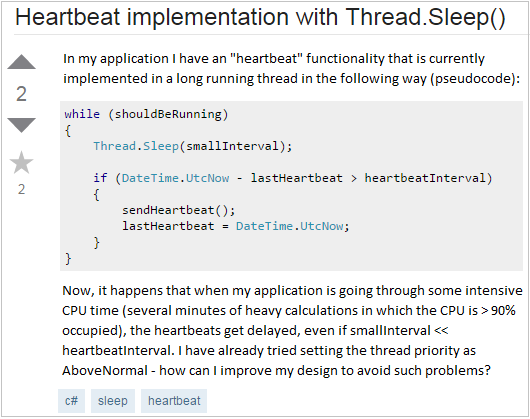
\includegraphics[width=0.99\linewidth]{./img/Question}
%\caption{}
%\label{fig:Question}
%\end{figure}




%%%% DK: I removed this to protect blind review 9/19/15
% In a previous paper we presented the overall architecture of such search engine~\cite{BIGSE}.

Our primary contributions in this paper are:
%% DK: I put these into a list since I thought it would make it really clear what our contributions were and make them easy to read

\begin{enumerate}
   \setlength{\itemsep}{0pt} %Cut down on spacing for the different items in the list
   \setlength{\parskip}{0pt} %Cut down on spacing for the different items in the list
   \setlength{\parsep}{0pt}  %Cut down on spacing for the different items in the list

  \item Report the \textit{results of a qualitative code review study} conducted to identify challenges in implementing architectural tactics and \textit{reusing tactical code}.
  \item Identify the foundations of a practical tactic search engine.
  \item Introduce the notion of \textit{tactical clones} and formulate the next steps in realizing a tactic search engine.
\end{enumerate}


%A) Reporting the \textit{results of a qualitative code review study} conducted to identify challenges in implementing architectural tactics and \textit{reusing tactical code}. B) Identifying the foundations of a practical tactic search engine. C) Introducing the notion of \textit{tactical clones} and formulating the next steps in realizing tactic search engine.

Although there has been some initial development of source code recommender systems~\cite{DBLP:conf/icse/McMillanHPCM12,6340250}, the primary focus of this previous research is only on retrieving generic functional code and not tactical code. Therefore the challenges of obtaining and recommending tactical code is still unexplored. This paper focuses on identifying these challenges.

This paper organized as follows: Section~\ref{sec:Method} presents the underlying methodology used to conduct the qualitative study of tactic implementations. Section \ref{sec:SeenUnSeen} discusses the results of our qualitative study, tactic implementation issues, reusability concerns and other observations across several implementation of architectural tactics. This section also summarizes the foundations for developing a practical tactic search engine. Section \ref{sec:Clones} presents the definitions of tactical clones and the process of extracting sample architectural clones from source code of several open source systems. Section \ref{sec:Future} presents possible future work to build on our research and Section \ref{sec: relatedwork} discusses related works. Section \ref{sec:Conclusion} concludes our paper. 
